\begin{dfn}[Plane Geometry]
Let \(P\) be an ordered geometry with a segment congruence and an angle congruence.
We say that \(P\) is a \emph{plane geometry} if the following properties are satisfied.
\begin{proplist}
\item[PG1.] \textbf{Right Angle Property.} Any two right angles are congruent.

\item[PG2.] \textbf{Angle-Side Congruence.} Suppose \(a_1\), \(b_1\), and \(c_1\) are distinct points and \(a_2\), \(b_2\), and \(c_2\) are distinct points such that \(\SEGMENT{b_1}{a_1} \equiv \SEGMENT{b_2}{a_2}\) and \(\SEGMENT{b_1}{c_1} \equiv \SEGMENT{b_2}{c_2}\).
Then \(\SEGMENT{a_1}{c_1} \equiv \SEGMENT{a_2}{c_2}\) if and only if \(\ANGLE{a_1}{b_1}{c_1} \equiv \ANGLE{a_2}{b_2}{c_2}\).

\item[PG3.] \textbf{Circle Cut.} If \(o\), \(a\), and \(b\) are points such that \(a \neq o\) and \(b \neq o\), then there is a point \(c \in \RAY{o}{b}\) such that \(\SEGMENT{o}{c} \equiv \SEGMENT{o}{a}\).

\begin{center}
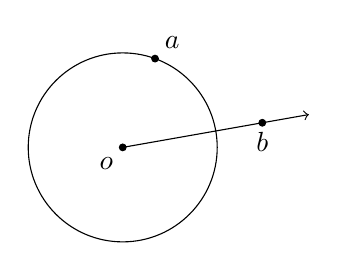
\begin{tikzpicture}[scale=0.6]
  \coordinate [label=below left:\(o\)]  (o) at (0  : 0);
  \draw [fill] (o) circle [radius=2pt];
  \coordinate [label=above right:\(a\)] (a) at (70 : 2);
  \draw [fill] (a) circle [radius=2pt];
  \coordinate [label=below:\(b\)]       (b) at (10 : 3);
  \draw [fill] (b) circle [radius=2pt];
  \draw [->] (o) -- (10: 4);
  \draw (o) circle [radius=2];
\end{tikzpicture}
\end{center}

\item[PG4.] \textbf{Interleaved Diameters.} Let \(C_1\) and \(C_2\) be circles centered at distinct points \(o_1\) and \(o_2\), respectively.
Further suppose we have diameters \(\SEGMENT{a_1}{b_1}\) of \(C_1\) and \(\SEGMENT{a_2}{b_2}\) of \(C_2\) such that \(\BETWEEN{a_1}{o_1}{a_2}\) and \(\BETWEEN{a_1}{o_2}{a_2}\).
Then \(C_1 \cap C_2\) is nonempty if and only if \(\BETWEENS{a_1b_2b_1a_2}\), and in this case \(C_1 \cap C_2\) consists of exactly two points which are on opposite sides of \(\LINE{o_1}{o_2}\).

\begin{center}
\begin{tikzpicture}[scale=0.7]
  \coordinate [label=above:{\(o_1\)}]  (o1) at (0,0);
  \draw [fill] (o1) circle [radius=2pt];
  \coordinate [label=above left:{\(a_1\)}] (a1) at ($ (o1)+(10 : -2) $);
  \draw [fill] (a1) circle [radius=2pt];
  \coordinate [label=above right:{\(b_1\)}] (b1) at ($ (o1)+(10 : 2) $);
  \draw [fill] (b1) circle [radius=2pt];
  \draw (o1) circle [radius=2];
  \coordinate [label=above:\(o_2\)]  (o2) at ($ (o1)+(10 : 4) $);
  \draw [fill] (o2) circle [radius=2pt];
  \coordinate [label=below right:\(a_2\)] (a2) at ($ (o2)+(10 : 3) $);
  \draw [fill] (a2) circle [radius=2pt];
  \coordinate [label=below left:\(b_2\)] (b2) at ($ (o2)+(10 : -3) $);
  \draw [fill] (b2) circle [radius=2pt];
  \draw (o2) circle [radius=3];
  \draw [<->] ($ (o1)+(10 : -3) $) -- ($ (o2)+(10 : 4) $);
\end{tikzpicture}
\end{center}
\end{proplist}
\end{dfn}

Each of these properties says something which is (hopefully!) fairly intuitive.
Angle-Side Congruence provides an essential link between segment congruence and angle congruence, which are otherwise unrelated.
The Circle Cut and Interleaved Diameters properties allow us to construct points on the intersection of a circle with a central ray and of two circles, respectively.
(Without these we have no way to construct points on circles!)

We finally have enough technology to start doing some more recognizable geometry.
For the remainder of this chapter \(P\) is a plane geometry.
First, we give two shortcut results for determining when two triangles are congruent.

\begin{prop}[SSS Theorem]\label{prop:sss-theorem}
If two nondegenerate triangles can be labeled such that corresponding sides are congruent, then the triangles are congruent.

More precisely, let \(a_1\), \(b_1\), and \(c_1\) be distinct points and \(a_2\), \(b_2\), and \(c_2\) be distinct points.
If \(\SEGMENT{a_1}{b_1} \equiv \SEGMENT{a_2}{b_2}\), \(\SEGMENT{b_1}{c_1} \equiv \SEGMENT{b_2}{c_2}\), and \(\SEGMENT{c_1}{a_1} \equiv \SEGMENT{c_2}{a_2}\), then \(\TRIANGLE{a_1}{b_1}{c_1} \equiv \TRIANGLE{a_2}{b_2}{c_2}\).
\end{prop}

\begin{proof}
We have \(\ANGLE{a_1}{b_1}{c_1} \equiv \ANGLE{a_2}{b_2}{c_2}\), \(\ANGLE{b_1}{c_1}{a_1} \equiv \ANGLE{b_2}{c_2}{a_2}\), and \(\ANGLE{c_1}{a_1}{b_1} \equiv \ANGLE{c_2}{a_2}{b_2}\) using the Angle-Side Congruence property three times.
\end{proof}

\begin{prop}[SAS Theorem]\label{prop:sas-theorem}
If two nondegenerate triangles can be labeled such that two corresponding sides, and the angles between, are congruent, then the triangles are congruent.

More precisely, let \(a_1\), \(b_1\), and \(c_1\) be distinct points, and \(a_2\), \(b_2\), and \(c_2\) be distinct points.
If \(\SEGMENT{a_1}{b_1} \equiv \SEGMENT{a_2}{b_2}\), \(\SEGMENT{b_1}{c_1} \equiv \SEGMENT{b_2}{c_2}\), and \(\ANGLE{a_1}{b_1}{c_1} \equiv \ANGLE{a_2}{b_2}{c_2}\), then \(\TRIANGLE{a_1}{b_1}{c_1} \equiv \TRIANGLE{a_2}{b_2}{c_2}\).
\end{prop}

\begin{proof}
We have \(\SEGMENT{a_1}{c_1} \equiv \SEGMENT{a_2}{c_2}\) by Angle-Side Congruence, and then \hyperref[prop:sss-theorem]{SSS} applies.
\end{proof}

\begin{cor}[Pons Asinorum]\label{cor:pons-asinorum}
If \(\TRIANGLE{a}{b}{c}\) is isoceles with \(\SEGMENT{a}{b} \equiv \SEGMENT{b}{c}\), then \(\ANGLE{b}{a}{c} \equiv \ANGLE{b}{c}{a}\).
\end{cor}

\begin{proof}
We have two triangles, \(\TRIANGLE{b}{a}{c}\) and \(\TRIANGLE{b}{c}{a}\), such that \(\SEGMENT{b}{c}\equiv \SEGMENT{b}{a}\), \(\SEGMENT{b}{a} \equiv \SEGMENT{b}{c}\), and \(\ANGLE{c}{b}{a} \equiv \SEGMENT{a}{b}{c}\).
By \hyperref[prop:sas-theorem]{SAS} we have \(\TRIANGLE{b}{a}{c} \equiv \TRIANGLE{b}{c}{a}\), and thus \(\ANGLE{b}{a}{c} \equiv \ANGLE{b}{c}{a}\) as needed.
\end{proof}

\begin{cor}
Every triangle which is equilateral is also equiangular; all three interior angles are congruent.
\end{cor}

\begin{proof}
Follows from two applications of Pons Asinorum.
\end{proof}

\begin{cor}[Segment Addition]\label{cor:segment-addition}
Suppose \(\BETWEEN{a_1}{b_1}{c_1}\) and \(\BETWEEN{a_2}{b_2}{c_2}\).
If any two of \(\SEGMENT{a_1}{b_1} \equiv \SEGMENT{a_2}{b_2}\), \(\SEGMENT{b_1}{c_1} \equiv \SEGMENT{b_2}{c_2}\), and \(\SEGMENT{a_1}{c_1} \equiv \SEGMENT{a_2}{c_2}\) hold, then so does the third.
\end{cor}

\begin{proof}
Note that \(\ANGLE{a_1}{b_1}{c_1} \equiv \ANGLE{a_2}{b_2}{c_2}\), \(\ANGLE{b_1}{c_1}{a_1} \equiv \ANGLE{b_2}{c_2}{a_2}\), and \(\ANGLE{c_1}{a_1}{b_1} \equiv \ANGLE{c_2}{a_2}{b_2}\) by AC1.
The result then follows from three applications of \hyperref[prop:sas-theorem]{SAS}.
\end{proof}

\begin{dfn}[Antipode]
Let \(a\), \(b\), and \(c\) be points.
We say that \(c\) is an \emph{antipode}\index{antipode} of \(a\) \emph{through} \(b\) if \(\BETWEEN{a}{b}{c}\) and \(\SEGMENT{a}{b} \equiv \SEGMENT{b}{c}\).
\end{dfn}

\begin{construct}[Antipode]\label{construct:antipode}
Given distinct points \(a\) and \(b\), there is a unique point \(c\) such that \(c\) is an antipode of \(a\) through \(b\).
\end{construct}

\begin{proof}
First we show existence.
Using the Interpolation property, there is a point \(u\) such that \(\BETWEEN{u}{b}{a}\).
Now using Circle Cut, there is a point \(c \in \RAY{b}{u} \cap \CIRCLE{b}{a}\).
Note that \(\BETWEEN{a}{b}{c}\), and we have \(\SEGMENT{b}{c} \equiv \SEGMENT{b}{a}\) as needed.
Next we show uniqueness.
Suppose \(d\) is a point such that \(\BETWEEN{a}{b}{d}\) and \(\SEGMENT{a}{b} \equiv \SEGMENT{b}{d}\).
But then \(d \in \RAY{b}{c}\), and in fact \(c = d\) by AC4.
\end{proof}

\begin{construct}[Equilateral triangle with a given side]\label{construct:equilateral-points}
Given distinct points \(a\) and \(b\), there exist points \(c_1\) and \(c_2\), on opposite sides of \(\LINE{a}{b}\), such that \(\TRIANGLE{a}{b}{c_1}\) and \(\TRIANGLE{a}{b}{c_2}\) are equilateral.
In fact, we have \(\TRIANGLE{a}{b}{c_1} \equiv \TRIANGLE{a}{b}{c_2}\).
\end{construct}

\begin{proof}
First, construct the antipode \(h\) of \(b\) through \(a\), and construct the antipode \(k\) of \(a\) through \(b\).
Note that \(\BETWEENS{habk}\), and that \(\SEGMENT{a}{h} \equiv \SEGMENT{a}{b}\) and \(\SEGMENT{b}{k} \equiv \SEGMENT{b}{a}\); that is, \(a\) is a midpoint of \(\SEGMENT{h}{b}\) and \(b\) a midpoint of \(\SEGMENT{a}{k}\), so that \(a\) is the center of \(\CIRCLE{a}{b}\) with diameter \(\SEGMENT{h}{b}\) and \(b\) is the center of \(\CIRCLE{b}{a}\) with diameter \(\SEGMENT{a}{k}\).
Thus the Interleaved Diameters property applies, and we have two points \(c_1,c_2 \in \CIRCLE{a}{b} \cap \CIRCLE{b}{a}\) which are in opposite halfplanes of \(\LINE{a}{b}\).
Note that \(\SEGMENT{a}{c_1} \equiv \SEGMENT{a}{b} \equiv \SEGMENT{b}{c_1}\), and thus \(\TRIANGLE{a}{b}{c_1}\) is equilateral.
Similarly, \(\TRIANGLE{a}{b}{c_2}\) is equilateral.
Moreover, we see that \(\TRIANGLE{a}{b}{c_1} \equiv \TRIANGLE{a}{b}{c_2}\) by the SSS Theorem.
\end{proof}

\begin{lem}[Betweenness Transfer]\label{lem:betweenness-transfer}
Let \(a_1\), \(b_1\), \(c_1\), \(a_2\), \(b_2\), and \(c_2\) be points such that \(\BETWEEN{a_1}{b_1}{c_1}\), \(b_2 \in \RAY{a_2}{c_2}\), \(\SEGMENT{a_1}{b_1} \equiv \SEGMENT{a_2}{b_2}\), and \(\SEGMENT{a_1}{c_1} \equiv \SEGMENT{a_2}{c_2}\).
Then \(\BETWEEN{a_2}{b_2}{c_2}\).
\end{lem}

\begin{proof}
Note that \(a_1\), \(b_1\), and \(c_1\) are distinct.
Since \(\SEGMENT{a_1}{b_1} \equiv \SEGMENT{a_2}{b_2}\), \(a_2\) and \(b_2\) are distinct.
If \(b_2 = c_2\), then we have \(\SEGMENT{a_1}{b_1} \equiv \SEGMENT{a_1}{c_1}\), so that \(b_1 = c_1\) by S3 -- a contradiction.
So \(b_2\) and \(c_2\) are distinct.
Because \(b_2 \in \RAY{a_2}{c_2}\), there are two possibilities: either \(\BETWEEN{a_2}{c_2}{b_2}\) or \(\BETWEEN{a_2}{b_2}{c_2}\).

Suppose \(\BETWEEN{a_2}{c_2}{b_2}\).
Now \(\ANGLE{c_2}{a_2}{b_2} \equiv \ANGLE{c_1}{a_1}{b_1}\) (both angles are flat), and by \hyperref[prop:sas-theorem]{SAS} we have \(\TRIANGLE{c_1}{a_1}{b_1} \equiv \TRIANGLE{c_2}{a_2}{b_2}\).
In particular, we have \(\ANGLE{a_1}{b_1}{c_1} \equiv \ANGLE{a_2}{b_2}{c_2}\); a contradiction, as in this case \(\ANGLE{a_1}{b_1}{c_1}\) is straight while \(\ANGLE{a_2}{b_2}{c_2}\) is flat.
Thus \(\BETWEEN{a_2}{b_2}{c_2}\) as claimed.
\end{proof}

\begin{construct}[Segment Copy Theorem]
Let \(a\) and \(b\) be distinct points, and let \(o\) and \(t\) be distinct points.
Then there is a unique point \(x\) on \(\RAY{o}{t}\) such that \(\SEGMENT{o}{x} \equiv \SEGMENT{a}{b}\).
\end{construct}

\begin{proof}
First we construct a point \(z\) such that \(\TRIANGLE{a}{o}{z}\) is equilateral; now \(\SEGMENT{z}{a} \equiv \SEGMENT{z}{o}\).
Using the Interpolation property, construct a point \(h\) such that \(\BETWEEN{z}{a}{h}\), and using the Circle Cut property, construct a point \(u\) on \(\RAY{a}{h}\) such that \(\SEGMENT{a}{u} \equiv \SEGMENT{a}{b}\).
Again using Circle Cut, construct a point \(v\) on \(\RAY{z}{o}\) such that \(\SEGMENT{z}{v} \equiv \SEGMENT{z}{u}\).
By \lemref{lem:betweenness-transfer} we have \(\BETWEEN{z}{o}{v}\).
Now \(\SEGMENT{z}{a} \equiv \SEGMENT{z}{o}\) and \(\SEGMENT{z}{u} \equiv \SEGMENT{z}{v}\), thus \(\SEGMENT{a}{u} \equiv \SEGMENT{o}{v}\).
Again using Circle Cut, construct a point \(x\) on \(\RAY{o}{t}\) such that \(\SEGMENT{o}{x} \equiv \SEGMENT{o}{v}\).
Then we have \(\SEGMENT{o}{x} \equiv \SEGMENT{o}{v} \equiv \SEGMENT{a}{u} \equiv \SEGMENT{a}{b}\) as needed.
Uniqueness follows from SC3.
\end{proof}

\begin{construct}[Angle Copy Theorem]
Let \(a\), \(o\), \(b\) be distinct noncollinear points and let \(p\) and \(x\) be distinct points.
There exist two points \(y_1\) and \(y_2\), on opposite sides of \(\LINE{p}{x}\), such that \(\ANGLE{x}{p}{y_1} \equiv \ANGLE{x}{p}{y_2} \equiv \ANGLE{a}{o}{b}\). 
\end{construct}

\begin{proof}
First copy segment \(\SEGMENT{o}{b}\) onto \(\RAY{p}{x}\) at the point \(u\), then copy the segment \(\SEGMENT{b}{a}\) onto the ray \(\RAY{u}{p}\) at the point \(v\).
Now copy \(\SEGMENT{o}{a}\) onto \(\RAY{p}{x}\) at the point \(w\).
Note that \(\SEGMENT{o}{a} \equiv \SEGMENT{p}{w}\), \(\SEGMENT{o}{b} \equiv \SEGMENT{p}{u}\), and \(\SEGMENT{b}{a} \equiv \SEGMENT{u}{v}\).
Moreover, the intersection \(\CIRCLE{o}{a} \cap \CIRCLE{b}{a}\) is nonempty, as it contains \(a\).
By the Interleaved Diameters property, \(\CIRCLE{p}{w} \cap \CIRCLE{u}{v}\) contains two points \(z_1\) and \(z_2\) on opposite sides of \(\LINE{p}{x}\).
By the SSS Theorem, we have \(\TRIANGLE{p}{u}{z_1} \equiv \TRIANGLE{o}{b}{a} \equiv \TRIANGLE{p}{u}{z_2}\), and thus \(\ANGLE{u}{p}{z_1} \equiv \ANGLE{a}{o}{b} \equiv \ANGLE{u}{p}{z_2}\) as needed.
\end{proof}

\begin{prop}[ASA Theorem]
Let \(a_1\), \(b_1\), and \(c_1\) be distinct noncollinear points, and let \(a_2\), \(b_2\), and \(c_2\) be distinct points.
If \(\ANGLE{a_1}{b_1}{c_1} \equiv \ANGLE{a_2}{b_2}{c_2}\), \(\SEGMENT{b_1}{c_1} \equiv \SEGMENT{b_2}{c_2}\), and \(\ANGLE{b_1}{c_1}{a_1} \equiv \ANGLE{b_2}{c_2}{a_2}\), then \(\TRIANGLE{a_1}{b_1}{c_1} \equiv \TRIANGLE{a_2}{b_2}{c_2}\).
\end{prop}

\begin{proof}
Copy \(\SEGMENT{b_2}{a_2}\) onto \(\RAY{b_1}{a_1}\) at \(d\).
Note that \(d\) and \(a_1\) are on the same side of \(\LINE{b_1}{c_1}\).
Moreover, we have \(\TRIANGLE{d}{b_1}{c_1} \equiv \TRIANGLE{a_2}{b_2}{c_2}\) by \hyperref[prop:sas-theorem]{SAS}, and so \(\ANGLE{b_1}{c_1}{d} \equiv \ANGLE{b_2}{c_2}{a_2} \equiv \ANGLE{b_1}{c_1}{a_1}\).
By AC4, we have \(d \in \RAY{c_1}{a_1}\).
Now \(d\) is on both \(\LINE{b_1}{a_1}\) and \(\LINE{c_1}{a_1}\), and since \(a_1\), \(b_1\), and \(c_1\) are not collinear, we must have \(d = a_1\).
So we have \(\TRIANGLE{a_1}{b_1}{c_1} \equiv \TRIANGLE{a_2}{b_2}{c_2}\) as claimed.
\end{proof}
